\begin{figure}[H]
	\begin{center}
		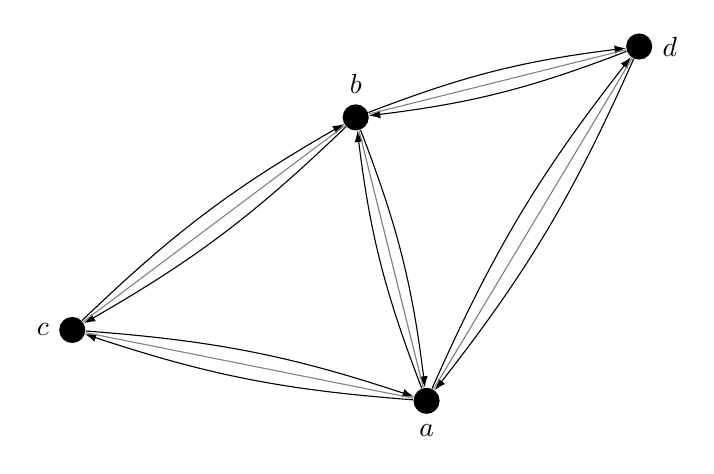
\begin{tikzpicture}[scale=0.9]
		\node [fill,circle,label=below:$a$] (A) at (6,1){};
		\node [fill,circle,label=above:$b$] (B) at (5,5){};
		\node [fill,circle,label=left: $c$] (C) at (1,2){};
		\node [fill,circle,label=right:$d$] (D) at (9,6){};
		\path[->,>=latex]
		(A) edge [bend left=7](B)
		(B) edge [bend left=7](C)
		(C) edge [bend left=7](B)
		(C) edge [bend left=7](A)
		(A) edge [bend left=7](C)
		
		(B) edge [bend left=7](A)
		(A) edge [bend left=7](D)
		(D) edge [bend left=7](B)
		(D) edge [bend left=7](A)
		(B) edge [bend left=7](D)
		;
		
		\path[-,color=gray]
		(A) edge (B)
		(B) edge (C)
		(C) edge (A)
		(A) edge (D)
		(D) edge (B)		
		;
		\end{tikzpicture}
	\end{center}
	\caption{Example of a Representation of the Half-Edge Structure}
	\label{fig:hedge}
\end{figure}